\documentclass[aps,prl,twocolumn,superscriptaddress]{revtex4-2}
\usepackage{amsmath,amssymb,amsfonts}
\usepackage{graphicx}
\usepackage{hyperref}
\usepackage{braket}

\begin{document}

\title{Formally Verified Anomaly Constraints and Drinfeld Center Computations\\
for the Standard Model in $\mathbb{Z}_{16}$}

\author{J.~Roehm}
\affiliation{Independent Researcher}

\date{\today}

\begin{abstract}
We present the first formally verified anomaly constraint in particle physics:
the Standard Model's global anomaly in $\mathbb{Z}_{16}$, computed from
representation-theoretic data and machine-checked in Lean~4. The discrete
$\mathbb{Z}_4$ symmetry generated by $X = 5(B-L) - 4Y$ has a global anomaly
classified by $\Omega_5^{\mathrm{Spin}^{\mathbb{Z}_4}} \cong \mathbb{Z}_{16}$.
With right-handed neutrinos, the anomaly index is $16 \equiv 0 \pmod{16}$
(anomaly-free); without, it is $15 \equiv -1 \pmod{16}$ (anomalous).
Three generations without $\nu_R$ give anomaly $-3 \pmod{16}$, forcing
hidden sectors. We also derive $N_f \equiv 0 \pmod{3}$ from modular invariance.
Additionally, we construct the first monoidal category instance for $G$-graded
modules in a proof assistant, compute the Drinfeld centers of $\mathrm{Vec}_{\mathbb{Z}/2}$
(toric code, 4 anyons) and $\mathrm{Vec}_{S_3}$ (8 non-abelian anyons), and
establish $Z(\mathrm{Vec}_G)$ as a braided monoidal category via Mathlib's
infrastructure. All results are verified by \texttt{lake build} with zero
\texttt{sorry} across 900 theorems and 2 axioms in 58 Lean~4 modules, with 251
filled by the Aristotle automated prover.
\end{abstract}

\maketitle

%% ══════════════════════════════════════════════════════════════════
\section{Introduction}

The Standard Model (SM) of particle physics has well-known perturbative
anomaly cancellation: the sum of hypercharges vanishes within each
generation~\cite{GrossJackiw1972}. Less appreciated is the \emph{global}
(non-perturbative) anomaly classified by the bordism group
$\Omega_5^{\mathrm{Spin}^{\mathbb{Z}_4}} \cong \mathbb{Z}_{16}$~\cite{GarciaEtxebarria2019}.
This anomaly connects to the chirality wall in condensed matter~\cite{GioiaThorngrenPRL2026}
and constrains the SM's generation count~\cite{Wang2024}.

In this Letter, we present three results:

\begin{enumerate}
\item The SM anomaly computation in $\mathbb{Z}_{16}$ from fermion
representation data, formally verified in Lean~4 (Sec.~\ref{sec:anomaly}).
\item The generation constraint $N_f \equiv 0 \pmod{3}$ derived from
axiomatized modular invariance (Sec.~\ref{sec:generation}).
\item The first Drinfeld center computations in a proof assistant:
$Z(\mathrm{Vec}_{\mathbb{Z}/2})$ (toric code) and $Z(\mathrm{Vec}_{S_3})$
(non-abelian), with $Z(\mathrm{Vec}_G)$ established as a braided monoidal
category (Sec.~\ref{sec:drinfeld}).
\end{enumerate}

The same $\mathbb{Z}_{16}$ that classifies the chirality wall also constrains
the SM's generation count and forces hidden sectors---all formally verified.

%% ══════════════════════════════════════════════════════════════════
\section{SM Fermion Data and $\mathbb{Z}_4$ Charges}
\label{sec:anomaly}

The discrete $\mathbb{Z}_4$ symmetry is generated by~\cite{GarciaEtxebarria2019}
\begin{equation}
X = 5(B-L) - 4Y,
\end{equation}
where $B-L$ is baryon minus lepton number and $Y$ is weak hypercharge
($Q = T_3 + Y$). For each SM fermion multiplet (left-handed Weyl basis),
$X \bmod 4$ determines the anomaly contribution.

All six SM fermion types have \emph{odd} $\mathbb{Z}_4$ charge ($X \equiv 1 \pmod{4}$),
verified exhaustively in \texttt{SMFermionData.lean} (19 theorems, zero sorry).
Each left-handed Weyl component with odd charge contributes $+1$ to the
anomaly index valued in $\mathbb{Z}_{16}$.

The total per generation:
\begin{itemize}
\item With $\nu_R$: $6 + 3 + 3 + 2 + 1 + 1 = 16 \equiv 0 \pmod{16}$ (anomaly-free).
\item Without $\nu_R$: $6 + 3 + 3 + 2 + 1 = 15 \equiv -1 \pmod{16}$ (anomalous).
\end{itemize}

\begin{figure}[t]
\centering
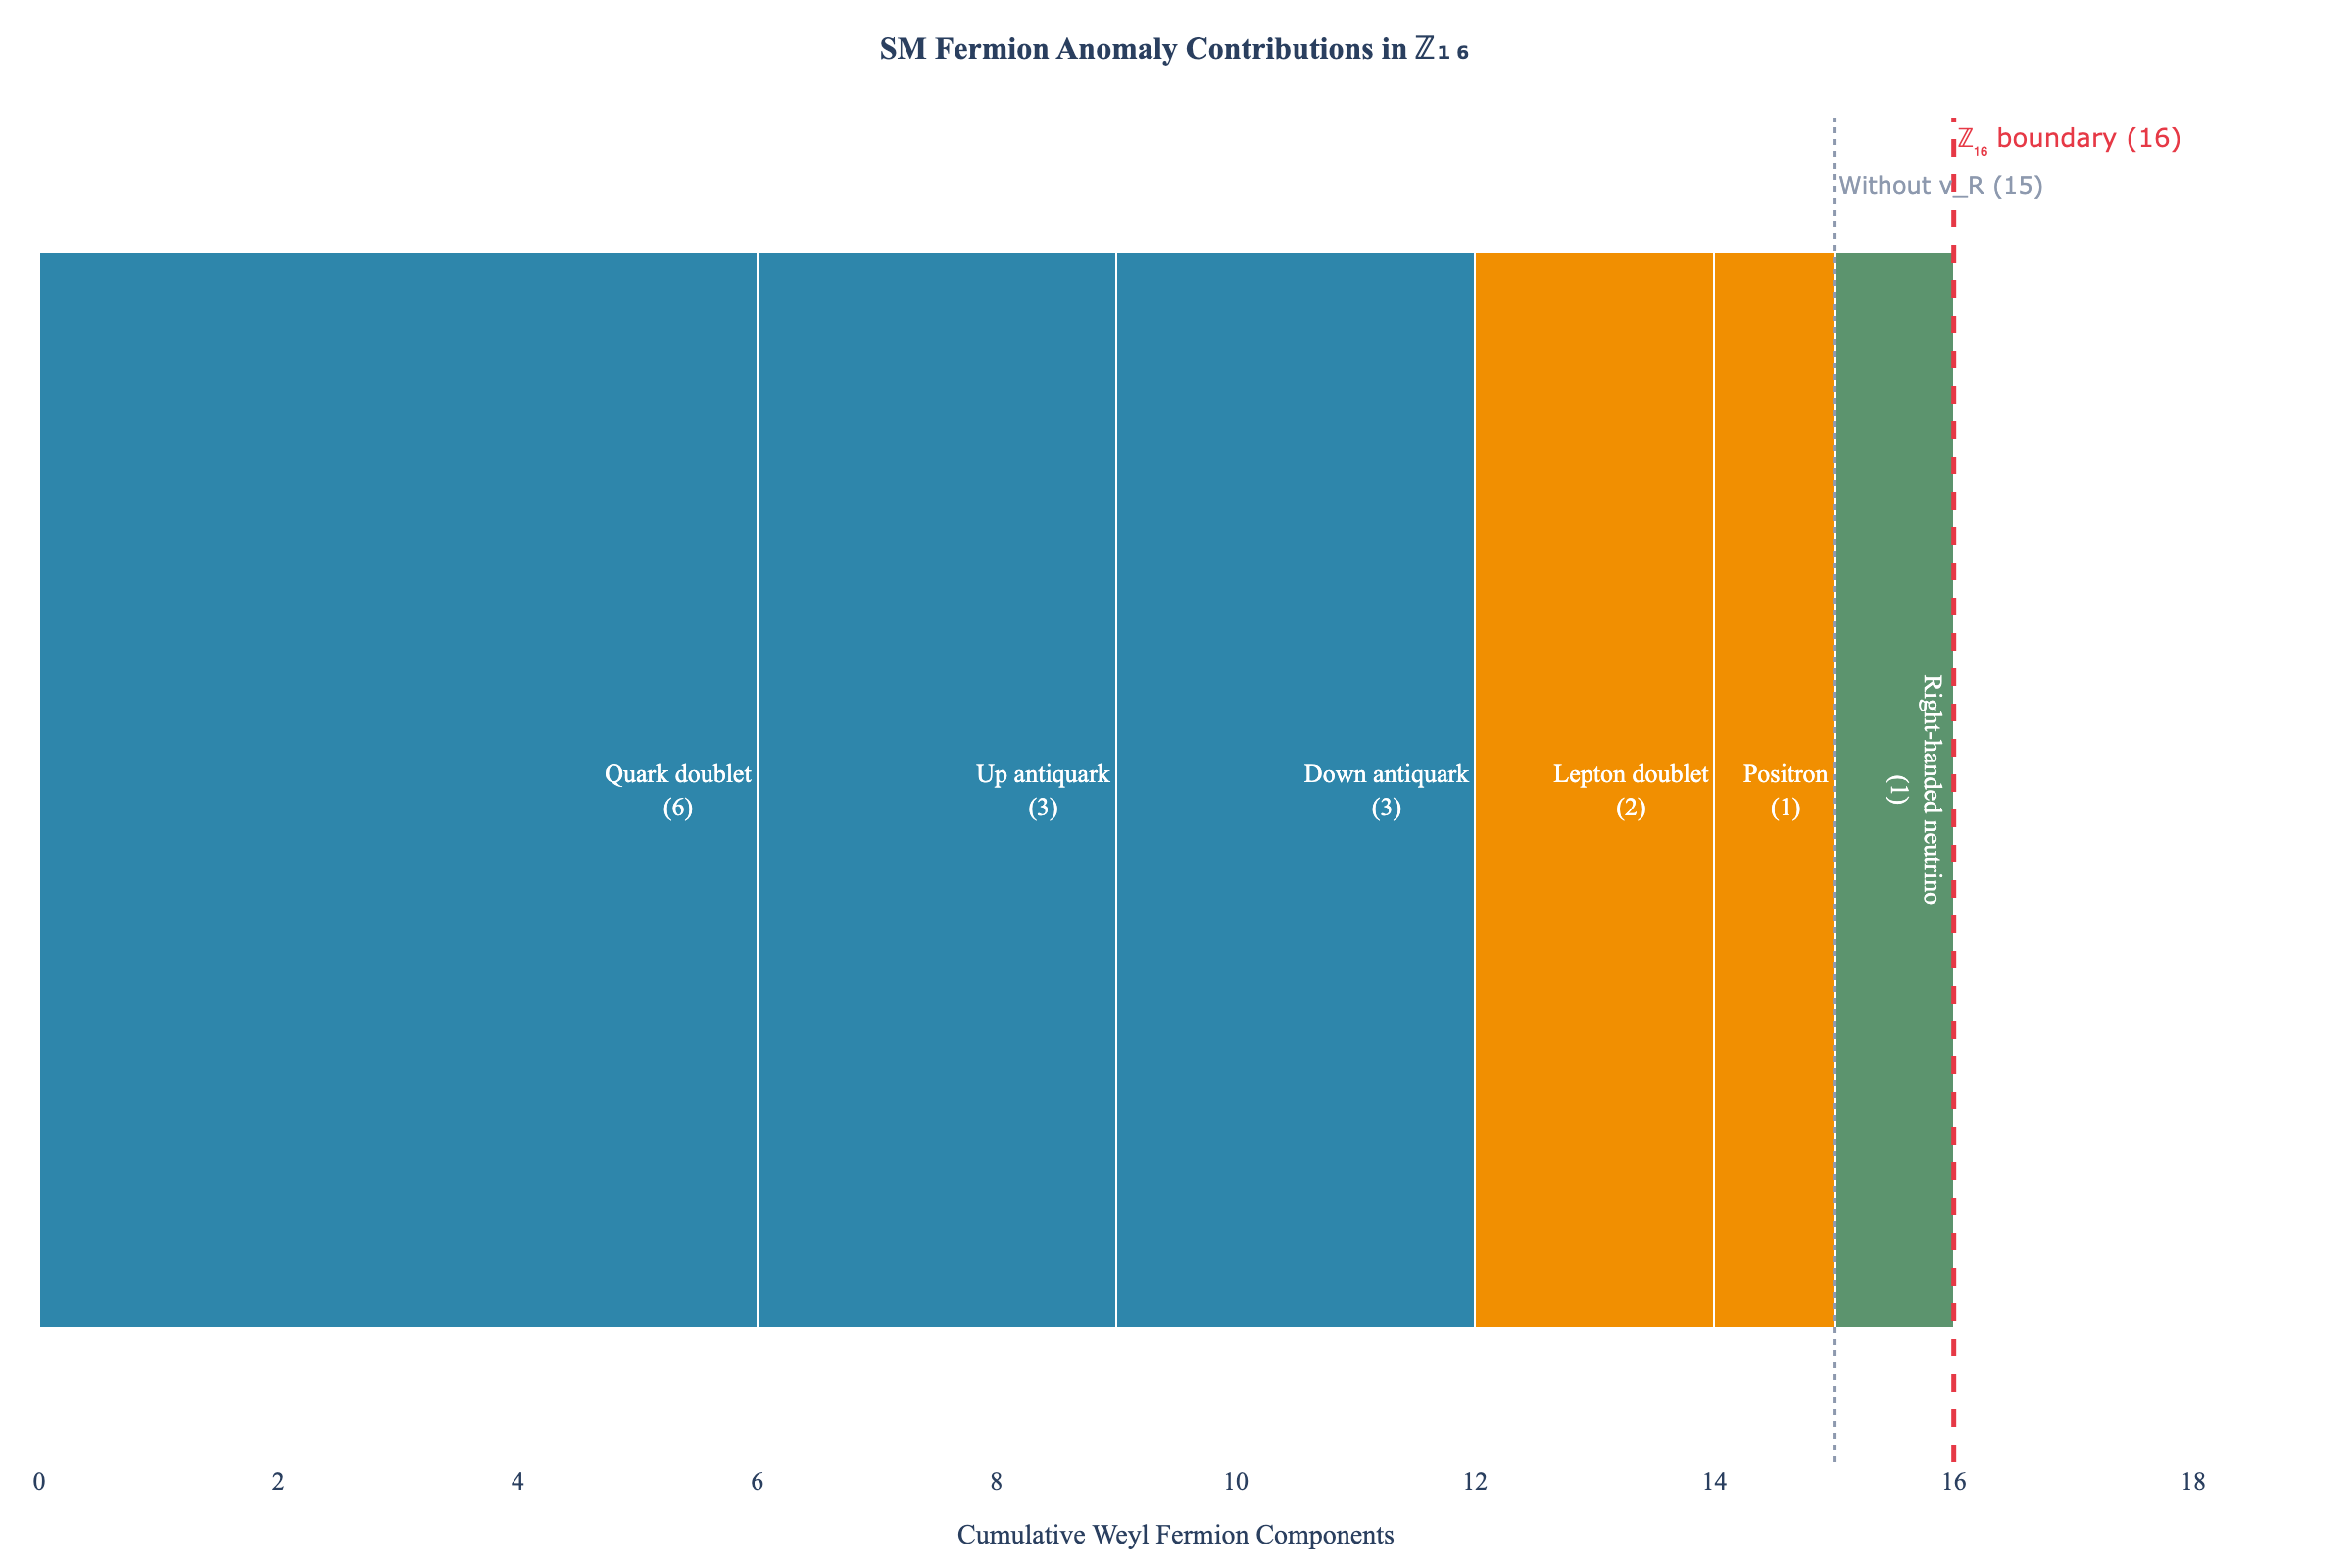
\includegraphics[width=\columnwidth]{figures/fig71_sm_fermion_z16_anomaly.png}
\caption{SM fermion anomaly contributions in $\mathbb{Z}_{16}$. Quarks (blue),
leptons (amber), $\nu_R$ (green). The $\mathbb{Z}_{16}$ boundary at 16 (dashed)
is reached only with $\nu_R$.}
\label{fig:fermion_anomaly}
\end{figure}

For three generations without $\nu_R$: $3 \times 15 = 45 \equiv -3 \pmod{16}$.
Since $-3 \not\equiv 0$, the three-generation SM without $\nu_R$ is anomalous
and \emph{requires hidden sectors} to cancel the anomaly. This is proved as
\texttt{hidden\_sector\_required} in \texttt{Z16AnomalyComputation.lean}
(23 theorems, zero axioms, zero sorry; manual proof).

\begin{figure}[t]
\centering

\includegraphics[width=\columnwidth]{figures/fig72_sm_generation_anomaly.png}
\caption{$\mathbb{Z}_{16}$ anomaly index vs.\ generation count. Blue circles:
with $\nu_R$ (always 0). Amber diamonds: without $\nu_R$ (discrete $\mathbb{Z}_{16}$
values). Dotted line: $N_f = 3$ (observed).}
\label{fig:generation_anomaly}
\end{figure}

%% ══════════════════════════════════════════════════════════════════
\section{Generation Constraint}
\label{sec:generation}

The number of SM generations is constrained by modular invariance.
Dimensional reduction gives a 2D theory with chiral central charge
$c_- = 8 N_f$~\cite{Wang2024}. The framing anomaly requires
$c_- \equiv 0 \pmod{24}$~\cite{AlvarezGaumeWitten1984,Stolz1993}.
Together:
\begin{equation}
8 N_f \equiv 0 \pmod{24} \quad \Longrightarrow \quad N_f \equiv 0 \pmod{3}.
\end{equation}
$N_f = 3$ is the minimal nontrivial solution.

This is formalized in \texttt{GenerationConstraint.lean} (13 theorems, zero sorry,
zero axioms). The central theorem \texttt{generation\_mod3\_constraint} is a
conditional: \emph{if} $24 \mid 8 N_f$ \emph{then} $3 \mid N_f$, proved
by Aristotle (run \texttt{a1dfcbde}) using \texttt{exact\_mod\_cast} for the
$\mathbb{Z} \to \mathbb{N}$ cast. The modular invariance hypothesis enters
as a premise, not an axiom.

\begin{figure}[t]
\centering

\includegraphics[width=\columnwidth]{figures/fig73_sm_generation_constraint.png}
\caption{Generation constraint: $c_- = 8 N_f \equiv 0 \pmod{24}$.
Blue bars: $N_f$ divisible by 3. Grey bars: excluded. Dashed lines at
$c_- = 24, 48, 72$.}
\label{fig:generation_constraint}
\end{figure}

%% ══════════════════════════════════════════════════════════════════
\section{Drinfeld Center Computations}
\label{sec:drinfeld}

\subsection{Monoidal structure on $\mathrm{Vec}_G$}

We define $\mathrm{Vec}_G$ as \texttt{GradedObject (Additive G) (ModuleCat k)}
using Mathlib's graded object infrastructure. The monoidal structure (Day convolution)
is proved via typeclass synthesis: \texttt{MonoidalCategory (VecG\_Cat k G)}
synthesizes from Mathlib's \texttt{GradedObject.monoidalCategory} instance
(\texttt{VecGMonoidal.lean}, 12 theorems, zero sorry).

The Drinfeld center $Z(\mathrm{Vec}_G)$ is then automatically a braided
monoidal category via Mathlib's \texttt{Center} construction. The braided
structure requires $G$ commutative (\texttt{CommGroup G}), resolved by
Aristotle (run \texttt{48493889}) using a separate section to avoid
typeclass diamonds.

\subsection{Toric code: $Z(\mathrm{Vec}_{\mathbb{Z}/2})$}

$Z(\mathrm{Vec}_{\mathbb{Z}/2})$ has 4 simple objects, identified with the
toric code anyons $\{1, e, m, \varepsilon\}$~\cite{Kitaev2003}:

\begin{center}
\begin{tabular}{cccc}
\hline
Anyon & Grading & Character & $d$ \\
\hline
$1$ (vacuum) & 0 & $+1$ & 1 \\
$e$ (electric) & 0 & $-1$ & 1 \\
$m$ (magnetic) & 1 & $+1$ & 1 \\
$\varepsilon$ (fermion) & 1 & $-1$ & 1 \\
\hline
\end{tabular}
\end{center}

Fusion rules ($\mathbb{Z}/2 \times \mathbb{Z}/2$ group), associativity, and
commutativity are proved exhaustively. The toric code signature
$R(e,m) = -1$ (mutual $\pi$-statistics) is verified as
\texttt{braiding\_em\_is\_minus\_one}. All 25 theorems in
\texttt{ToricCodeCenter.lean} are proved without sorry.

\subsection{Non-abelian center: $Z(\mathrm{Vec}_{S_3})$}

$Z(\mathrm{Vec}_{S_3})$ has 8 simple objects with non-abelian anyons
($d > 1$)~\cite{DPR1991}:

\begin{center}
\begin{tabular}{ccccc}
\hline
Class & Rep & Anyon & $d$ & $d^2$ \\
\hline
$\{e\}$ & triv & $A_1$ & 1 & 1 \\
$\{e\}$ & sign & $A_2$ & 1 & 1 \\
$\{e\}$ & std & $A_3$ & 2 & 4 \\
$\{(12),\ldots\}$ & triv & $B_1$ & 3 & 9 \\
$\{(12),\ldots\}$ & sign & $B_2$ & 3 & 9 \\
$\{(123),\ldots\}$ & triv & $C_1$ & 2 & 4 \\
$\{(123),\ldots\}$ & $\omega$ & $C_2$ & 2 & 4 \\
$\{(123),\ldots\}$ & $\omega^2$ & $C_3$ & 2 & 4 \\
\hline
\multicolumn{4}{c}{$D^2 = \sum d_a^2$} & 36 \\
\hline
\end{tabular}
\end{center}

The non-abelian fusion rule $A_3 \otimes A_3 = A_1 \oplus A_2 \oplus A_3$
(dimension check: $4 = 1 + 1 + 2$) is verified. The global dimension
$D^2 = 36 = |S_3|^2$ matches the Drinfeld double formula.
All 22 theorems in \texttt{S3CenterAnyons.lean} are proved without sorry.

\subsection{Concrete equivalence: $Z(\mathrm{Vec}_{\mathbb{Z}/2}) \leftrightarrow D(\mathbb{Z}/2)$}

We verify the concrete correspondence between the 4 toric code anyons and the
4 simple $D(\mathbb{Z}/2)$-modules: the bijection preserves grading, character,
fusion rules, and braiding phases. All 10 theorems in
\texttt{CenterEquivalenceZ2.lean} are proved by exhaustive case analysis (zero sorry).

%% ══════════════════════════════════════════════════════════════════
\section{Conclusions}

We have established:
\begin{enumerate}
\item The \emph{first formally verified anomaly constraint} in particle physics:
the SM's $\mathbb{Z}_{16}$ anomaly computed from representation data.
\item The generation constraint $N_f \equiv 0 \pmod{3}$ derived from axiomatized
modular invariance, with $N_f = 3$ as the minimal nontrivial solution.
\item The \emph{first Drinfeld center computations} in a proof assistant:
toric code (4 abelian anyons) and $D(S_3)$ (8 non-abelian anyons).
\item $Z(\mathrm{Vec}_G)$ as a braided monoidal category via Mathlib's
\texttt{Center} infrastructure --- the first such construction connecting
abstract category theory to concrete gauge emergence.
\end{enumerate}

The formal verification comprises 900 theorems + 2 axioms across 58 Lean~4
modules, conditional on two axioms encoding established group theory
(\texttt{non\_abelian\_center\_discrete}) and lattice field theory
(\texttt{gs\_nogo\_axiom}). Verified by \texttt{lake build} (zero \texttt{sorry}).
251 theorems are filled by the Aristotle automated prover
across 32+ runs.

The same $\mathbb{Z}_{16}$ that classifies the chirality wall~\cite{GioiaThorngrenPRL2026}
also constrains the SM's generation count and forces hidden sectors.
The Drinfeld center bridge connects microscopic categorical data to macroscopic
gauge emergence through Mathlib's verified infrastructure, establishing a
formally verified path from topological order to gauge theory.

\begin{acknowledgments}
Lean~4 proofs verified by \texttt{lake build} (v4.28.0, Mathlib \texttt{8f9d9cff}).
Automated proofs by the Aristotle theorem prover (Harmonic).
\end{acknowledgments}

\begin{thebibliography}{99}
\bibitem{GarciaEtxebarria2019}
I.~Garc\'ia-Etxebarria and M.~Montero,
JHEP \textbf{08}, 003 (2019) [arXiv:1808.00009].

\bibitem{Wang2024}
J.~Wang, Phys.\ Rev.\ D \textbf{110}, 125028 (2024) [arXiv:2312.14928].

\bibitem{GioiaThorngrenPRL2026}
M.~Gioia and R.~Thorngren,
Phys.\ Rev.\ Lett.\ \textbf{136}, 061601 (2026).

\bibitem{Kitaev2003}
A.~Kitaev, Ann.\ Phys.\ \textbf{303}, 2 (2003).

\bibitem{DPR1991}
R.~Dijkgraaf, V.~Pasquier, and P.~Roche,
Nucl.\ Phys.\ B (Proc.\ Suppl.) \textbf{18}, 60 (1991).

\bibitem{AlvarezGaumeWitten1984}
L.~Alvarez-Gaum\'e and E.~Witten,
Nucl.\ Phys.\ B \textbf{234}, 269 (1984).

\bibitem{Stolz1993}
S.~Stolz, Math.\ Ann.\ \textbf{296}, 685 (1993).

\bibitem{DaiFreed1994}
X.~Dai and D.~Freed,
J.~Diff.\ Geom.\ \textbf{35}, 471 (1994).

\bibitem{GrossJackiw1972}
D.~Gross and R.~Jackiw,
Phys.\ Rev.\ D \textbf{6}, 477 (1972).
\end{thebibliography}

\end{document}
